% --
%
% Configuração do Documento
%
% --
\documentclass[10pt,brazil]{beamer}
\uselanguage{Portuguese}
\languagepath{Portuguese}
\usepackage[utf8]{inputenc}


% ---
% Pacotes adicionais
% ---
\usepackage[light,math]{kurier}         %Altera Fonte Utilizada no arquivo
\usepackage{amsmath,amsfonts,amsthm,amssymb,mathrsfs}
\allowdisplaybreaks[1]
\usepackage{microtype}
\usepackage{mathtools}
\usepackage{csquotes}
\usepackage{tikz}
\usetikzlibrary{matrix}
\usetikzlibrary{patterns}
\usepackage{faktor}
\usepackage[Sonny]{fncychap}
\usepackage{hyperref}
\usepackage{tikz}
\graphicspath{{images/}}
\usepackage[light,math]{kurier}
\usetheme{Madrid}
\useinnertheme{rectangles}


\renewcommand{\raggedright}{\leftskip=0pt \rightskip=0pt plus 0cm} %texto justificado

\usepackage[%
    alf,
    abnt-emphasize=bf,
    bibjustif,
    recuo=0cm,
    abnt-doi=expand,            % Expande um endereço iniciado com doi: para http://dx.doi.org/
    abnt-url-package=url,       % Utiliza o pacote url
    abnt-refinfo=yes,           % Utiliza o estilo bibliográfico abnt-refinfo
    abnt-etal-cite=3,
    abnt-etal-list=3,
    abnt-thesis-year=final
]{abntex2cite}   

\setbeamertemplate{theorems}[numbered] % to number
\setbeamercovered{transparent}

\theoremstyle{definition}
\newtheorem{dfn}{Definição}
\newtheorem{obs}{Observação}
\newtheorem*{proofthm}{Demonstração do Teorema}
\newtheorem*{proofprop}{Demonstração da Proposição}
\newtheorem{ex}{Exemplo}
\newtheorem{prop}{Propriedade}
\newtheorem{proposition}{Proposição}


\newcommand{\der}{\text{d}}					%Comando para fazer o d da derivada fora do ambienta matemático
\newcommand{\mb}[2]{\mathbb{#1}^{#2}}		%Comando para usar \mathbb de maneira  mais eficiente
\newcommand{\mca}[2]{\mathcal{#1}_{#2}}
\newcommand{\mul}[2]{\mu_{#1}\left(#2\right)}			%Comando para escrever a multiplicidade de modo mais eficiente
\newcommand{\mc}[2]{\mathcal{I}_{#1}\left(#2\right)}   %Comando para escrever o IPH de maneira  mais eficiente

% --
% Define Cores Personalizadas 
% --
\definecolor{ver}{RGB}{124,26,29}
\definecolor{yel}{RGB}{158,134,35}
\definecolor{ros}{RGB}{255,51,102}
\definecolor{ver1}{RGB}{169,88,99}
\definecolor{ver2}{RGB}{156,63,75}
\definecolor{ver3}{RGB}{145,43,56}
\definecolor{azul}{RGB}{18,35,97}

% --
% Customiza o título 
% --
\setbeamercolor{title}{fg=azul, bg=white!95!black}

% --
% Remove os controles de navegação 
% --
\setbeamertemplate{navigation symbols}{}

% --
% Customiza o background
% --
\setbeamertemplate{background}{
	\begin{tikzpicture}[remember picture,overlay]
	% --- LinhaInferior
	\draw[line width=0.4mm,azul] ([shift={(2.5cm,0.4cm)}]current page.south west) -- ([shift={(-0.38cm,0.4cm)}]current page.south east);
	\draw[line width=0.4mm,azul] ([shift={(-0.3cm,0.4cm)}]current page.south east) -- ([shift={(-0.26cm,0.4cm)}]current page.south east);
	\draw[line width=0.4mm,azul] ([shift={(2.75cm,0.3cm)}]current page.south west) -- ([shift={(-0.38cm,0.3cm)}]current page.south east);
	\draw[line width=0.4mm,azul] ([shift={(-0.3cm,0.3cm)}]current page.south east) -- ([shift={(-0.26cm,0.3cm)}]current page.south east);
	\draw[line width=0.4mm,azul] ([shift={(3cm,0.2cm)}]current page.south west) -- ([shift={(-0.38cm,0.2cm)}]current page.south east);
	\draw[line width=0.4mm,ver1] ([shift={(-0.3cm,0.2cm)}]current page.south east) -- ([shift={(-0.26cm,0.2cm)}]current page.south east);
	
	% --- Logo 
	\node[xshift=-1.5cm,yshift=-1cm] at (current page.north east) {
\includegraphics[scale=0.15]{logo_ufmg.jpg}};
	
	\end{tikzpicture}
}

% --
% Customiza o título do frame 
% --
\setbeamercolor{frametitle}{fg=azul, bg=white} 
\makeatletter
\setbeamertemplate{frametitle}
{
	\ifbeamercolorempty[bg]{frametitle}{}{\nointerlineskip}%
	\@tempdima=\textwidth%
	\advance\@tempdima by\beamer@leftmargin%
	\advance\@tempdima by\beamer@rightmargin%
	\pgfsetfillopacity{.1}       %<------ fix filling opacity
	\begin{beamercolorbox}[sep=0.3cm,left,wd=\the\@tempdima]{frametitle}
		\usebeamerfont{frametitle}%
		\vbox{}\vskip1ex \hskip6ex%
		\if@tempswa\else\csname beamer@fteleft\endcsname\fi%
		\strut\pgfsetfillopacity{1}\insertframetitle\strut\par%  <---- text opacity
		{%
			\ifx\insertframesubtitle\@empty%
			\else%
			{\usebeamerfont{framesubtitle}\usebeamercolor[fg]{framesubtitle}\insertframesubtitle\strut\par}%
			\fi
		}%
		\vskip-1ex%
		\if@tempswa\else\vskip-.3cm\fi% set inside beamercolorbox... evil here...
	\end{beamercolorbox}%
}
\makeatother


% --
% Customimza o ambiente de Teorema 
% --
\setbeamercolor{block title}{use=structure, fg=white, bg=azul}
\setbeamercolor{block body}{use=structure, fg=black, bg=white!96!black}
\setbeamertemplate{block begin}[default]
\setbeamertemplate{block end}[default]



% --
% Customiza o footline 
% --
\setbeamertemplate{footline}{}


% --
% Customiza o headline 
% --
\setbeamertemplate{headline}
{
	\leavevmode%
	\hbox{%
		\begin{beamercolorbox}[wd=\paperwidth,dp=3.5ex]{ver}%
			\raggedright
			\hspace*{2em}%
		\end{beamercolorbox}%
	}%
}


% --
% Customiza o estilo dos ambientes Itemize e Enumerate 
% --
\setbeamertemplate{enumerate item}{\color{azul}\insertenumlabel)}
\setbeamertemplate{enumerate subitem}{\color{azul}\insertenumlabel.\insertsubenumlabel)}
\setbeamertemplate{enumerate subsubitem}{\color{azul}\insertenumlabel.\insertsubenumlabel.\insertsubsubenumlabel)}
\setbeamertemplate{enumerate mini template}{\insertenumlabel}

\setbeamertemplate{itemize item}{\scriptsize\raise1.25pt\hbox{\color{azul}\donotcoloroutermaths$\bullet$}}
\setbeamertemplate{itemize subitem}{\tiny\raise1.5pt\hbox{\color{azul}\donotcoloroutermaths$\blacksquare$}}
\setbeamertemplate{itemize subsubitem}{\tiny\raise1.5pt\hbox{\color{azul}\donotcoloroutermaths$\blacktriangleright$}}

% -- 
% Customiza o estilo do Table of Contents 
% --
\setbeamertemplate{section in toc}[square]

\setbeamerfont{section number projected}{size=\large}
\setbeamercolor{section number projected}{bg=white!95!black, fg=azul}

\setbeamertemplate{subsection in toc}{%
	\leavevmode\leftskip=5.65ex%
	\llap{\raisebox{0.2ex}{\textcolor{azul}{$\bullet$}}\kern1ex}%
	\inserttocsubsection\par%
}

% -- 
%Customiza as margens dos frames 
% -- 
\setbeamersize{text margin left=1cm,text margin right=1cm}

% -- 
% Apresentação
% -- 
\begin{document}
\mode<presentation>

% -- 
% Info
% -- 
\title[]{ANÁLISE DE DADOS UTILIZANDO CLUSTER DE BAIXO CUSTO}
\subtitle{COMPARAÇÃO DE DESEMPENHO DE AMBIENTES VIRTUAIS}

\institute[UFMG]{Universidade Federal de Minas Gerais}

\author[Felipe Rocha]{Felipe Fonseca Rocha \\
  \vspace{0.25cm}
  Orientador: Ítalo Fernando Scotá Cunha}
\date{09 de Fevereiro de 2022}

% --
% Inclui o sumário antes de cada seção
% --
\AtBeginSection{%
  \begin{frame}
    \tableofcontents[currentsection, subsectionstyle=show/show/hide]
  \end{frame}
}
% -- 
% Cria slide com título
% -- 
\frame{\maketitle}

% -- 
% Cria slide com sumário
% -- 

\begin{frame}{Sumário}
  \tableofcontents[hideallsubsections]
\end{frame}

% 	\begin{figure}
% 		\centering
% 		\includegraphics[scale=0.45]{objetivo.jpg}
% 	\end{figure}

% --
%
% Conteúdo 
%
% --

% -- 
% Introdução
% -- 
\section{Introdução}

% -- 
% Introdução - Motivação
% -- 
\subsection{Introdução - Contexto e Motivação}

\begin{frame}[t,allowframebreaks]{Contexto e Motivação}
  \begin{columns}
    \begin{column}[t]{0.5\textwidth}
      \begin{itemize}
        \item[] A todo momento nós geramos milhoes de dados que são coletados por diferentes meios
        \item[] Várias ferramentas estão disponíveis para Transforma-los em informações e embasar descisões
      \end{itemize}
      %\cite{galvao_desafios_2019,mehta_concurrence_2018,brasildisponibilidade2016}
    \end{column}
    \begin{column}{0.5\textwidth}
      \begin{center}
        
\includegraphics[width=1\textwidth]{sis.png}
      \end{center}
    \end{column}
    \begin{column}{0.5\textwidth}
      
    \end{column}
  \end{columns}
  \framebreak
  \begin{columns}
    \begin{column}{0.5\textwidth}
      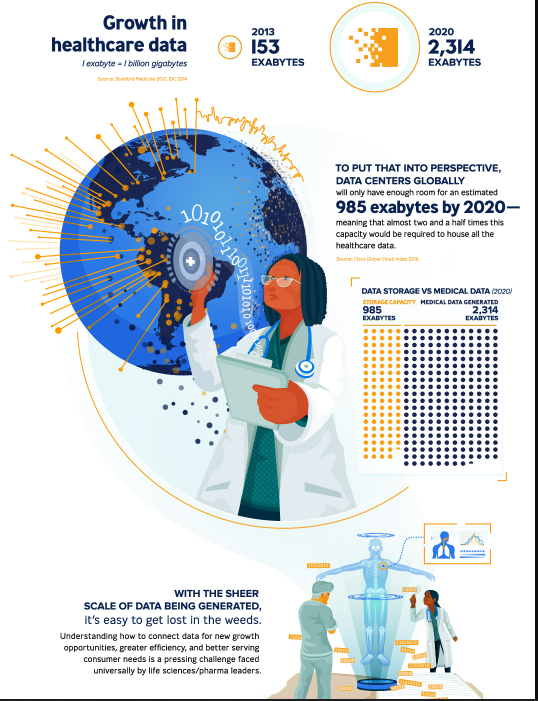
\includegraphics[width=1\textwidth,height=.75\textheight]{growthhealth.png}
    \end{column}
    \begin{column}[t]{0.6\textwidth}
      \begin{itemize}
        \item[] Isso também acontece na área da saúde
        \item[] Porém o uso dessas ferramentas nessa área, para transformar dados em informação, ainda é pouco significativo
      \end{itemize}
    \end{column}
  \end{columns}
  \framebreak
  %\begin{center}
  \begin{itemize}
    \item: Tendência crescente de trabalho interdisciplinar
    \item: Potencial de melhora do sistema de Saúde através de análise de dados
    \item: Necessário Propor e Validar estratégias que sejam viáveis e facilitem o processamento de analise de grande volume de dados produzido na área
  \end{itemize}
  %\end{center}
  \framebreak
  \begin{itemize}
    \item: No Brasil, dados do Sistema de Informação em Sáude (SIS) são disponibilizados desde 2016
    \item: \textbf{Faltam recursos} e Estratégias Viáveis para essa elboração.
  \end{itemize}
\end{frame}



% -- 
% Introdução - Justificava
% -- 
\subsection{Justificativa}

\begin{frame}{Introdução - Justificativa}
  \begin{columns}
    \begin{column}{0.5\textwidth}
      \begin{itemize}
        \item Restrição Orçamentária
              \begin{itemize}
                \item Diminuição de verbas para ciência e técnologia $-2,32\%$, mesmo com o aumento de base de alunos
                \item Aumento do dólar em mais de $3,27\%$ diminuindo o poder de compra
                \item Tomada de decisão em saúde, mais de 152mi de Brasileiros dependem exclusivamente do SUS %(UNASUS, 2021)
              \end{itemize}
        \item Necessidade de dispor estratégias de análise de dados
      \end{itemize}
    \end{column}
    \begin{column}{0.5\textwidth}  %%<--- here
      \begin{center}
        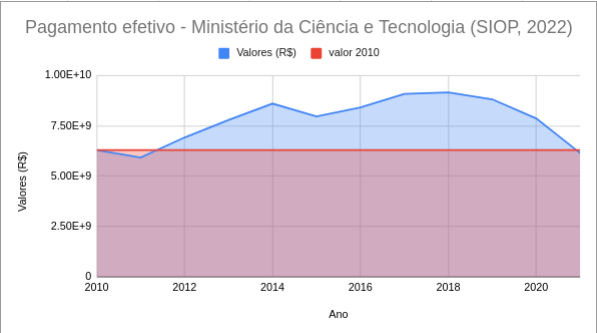
\includegraphics[width=1\textwidth]{orcamento.png}
        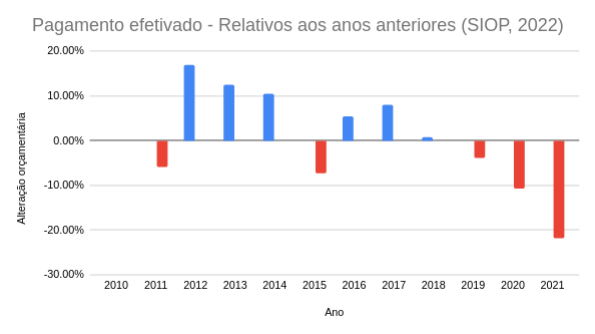
\includegraphics[width=1\textwidth]{variacaoorcamentaria.png}
      \end{center}
    \end{column}
  \end{columns}
\end{frame}

\begin{frame}{Introdução - Justificativa}
  \begin{columns}
    \begin{column}{0.5\textwidth}
      \begin{itemize}
        \item Restrição Orçamentária
              \begin{itemize}
                \item Diminuição de verbas para ciência e técnologia $-2,32\%$, mesmo com o aumento de base de alunos
                \item Aumento do dólar em mais de $3,27\%$ diminuindo o poder de compra
                \item Tomada de decisão em saúde, mais de 152mi de Brasileiros dependem exclusivamente do SUS %(UNASUS, 2021)
              \end{itemize}
        \item Necessidade de dispor estratégias de análise de dados
      \end{itemize}
    \end{column}
    \begin{column}{0.5\textwidth}  %%<--- here
      \begin{center}
        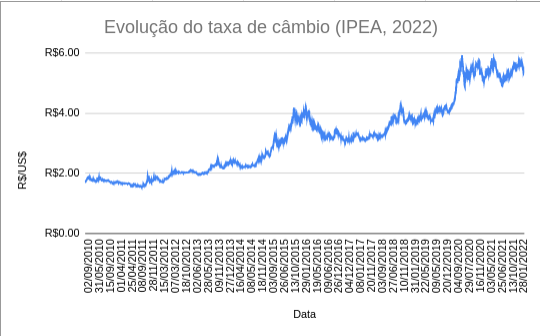
\includegraphics[width=1\textwidth]{variacaodolar.png}
      \end{center}
    \end{column}
  \end{columns}
\end{frame}

% -- 
% Introdução - Abordagem
% --
\subsection{Abordagem}
\begin{frame}{Introdução - Abordagem}
  Utilizar um Cluster Kubernetes como plataforma de orquestração de cargas de trabalho em ambiente virtual.
  \begin{itemize}
    \item Cargas de trabalho:
          \begin{itemize}
            \item Analise de tendencia de uso de azitromicina entre 2014 e 2021
          \end{itemize}
    \item Ambientes virtualizados (simulando \emph{Host} do cluster):
          \begin{itemize}
            \item completa - \emph{Hypervisor} tipo 2
            \item sistema operacional - contêineres
          \end{itemize}
          \framebreak
    \item Ambiente virtual:
          \begin{itemize}
            \item[] Simulação de máquina de baixo poder computacional:
            \item 1 vCPU
            \item 2 GB de RAM
            \item 6-8 máquinas
          \end{itemize}
  \end{itemize}
  Essa Abordagem visa comparar o desempenho desses ambientes simulados, e validar o uso de computadores de baixo poder computacional, no processo de análise de dados de grande volume
\end{frame}

\begin{frame}{Introdução - Abordagem}
  O uso de conceitos, métodose o uso de ferramentas complementares na aplicação da cultura DevOps em ambientes produtivos, permitirá o deployment simplificado melhorando a agilidade e diminuindo a complexidade e operação/sustentação do cluster
  \begin{itemize}
    \item Conceitos como:
          \begin{itemize}
            \item CI (integração contínua)
            \item CD (entrega contínua)
          \end{itemize}
    \item Uso do metodo USE (utilização, saturação e erro). Esse método propoe um checklist de métricas a serem coletadas e a avaliação de três paramêtros por meio dessas métricas, relacioando assim o performance da carga de trabalho (aplicação) e o desempenho dos nós do cluster sob monitoramento.
  \end{itemize}
\end{frame}


% -- 
% Objetivos
% -- 
\section{Objetivo}
%[allowframebreaks]
\begin{frame}{Objetivo}
  \begin{itemize}
    \item[] \textbf{Objetivos Geral:}
    \item[]
          \begin{itemize}
            \item[] Realizar a comparação de desempenho de orquestração de recursos em cluster de baixo custo em ambientes virtualizados, para o processamento e a análise dos dados.
          \end{itemize}
    \item[] \textbf{Objetivos Específicos:}
          \begin{itemize}
            \item Realizar a orquestração de recursos em cluster de baixo custo;
            \item Comparar o desempenho de clusters em ambientes virtualizados;
            \item Validar o uso de um cluster de utilização compartilhada para processamento de dados distribuídos;
            \item Propor um método de análise em cluster Kubernetes com uso de computadores desktops;
          \end{itemize}
          I\end{itemize}
\end{frame}


% -- 
% Revisão de Literatura
% -- 
\section{Revisão de literatura}

% -- 
% Revisão de Literatura - Análise de dados
% -- 
\subsection{Análise de dados}

\begin{frame}{Revisão de literatura- Análise de dados}
  \begin{itemize}
    \item Descisões em saúde costumam ser complexas - precisam de suporte científico (dados) e avaliação de Contexto
    \item Com o crescimento dos 3V's de dados na área da saúde (Big Data) processar e analisar esses dados tornouse fundamental para tomada de descisões adequadas
    \item Desafios:
          \begin{itemize}
            \item complexidade dos dados obtidos
            \item ausencia de validação de sistemas, métodos e ferramentas para o tratamento de dados na área
            \item custos de novos equipamentos capazes de analisar tal volume
          \end{itemize}
    \item Há grande oportunidade para a proposição de estratégias de processamento e anális de dados na área
  \end{itemize}
\end{frame}

% -- 
% Revisão de Literatura - Alternativas open source
% -- 
\subsection{Alternativas open source}

\begin{frame}{Revisão de literatura - Alternativas open source}
  \begin{itemize}
    \item Considerando
          \begin{itemize}
            \item O escopo deste trabalho
            \item As estratégias para processamento e análise de dados disponíveis no mercado
          \end{itemize}
    \item [] As soluções encontradas no mercado foram agrupadas em dois grupos:
          \begin{itemize}
            \item Soluções de Computação em nuvem privada:
                  \begin{itemize}
                    \item Se extendem para além do proposito desse trabalho
                    \item Requisitos de hardware elevados
                    \item Complexidade de configuração devido a sua abrangência
                  \end{itemize}
          \end{itemize}
  \end{itemize}
\end{frame}


\begin{frame}{Revisão de literatura- Alternativas open source}
  \begin{columns}
    \begin{column}{0.5\textwidth}
      \begin{itemize}
        \item Soluções de Orquestração de Containers:
              \begin{itemize}
                \item Kubernetes\textregistered
                \item Apache Mesos\textregistered
                \item Hashicorp Nomad\textregistered\*
                \item Docker Swarm\textregistered
              \end{itemize}
      \end{itemize}
    \end{column}
    \begin{column}{0.5\textwidth}  %%<--- here
      \begin{center}
        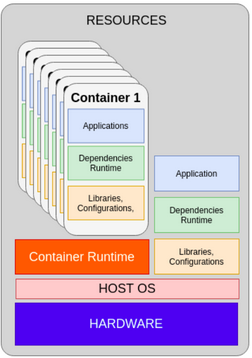
\includegraphics[width=0.5\textwidth]{containers.png}
        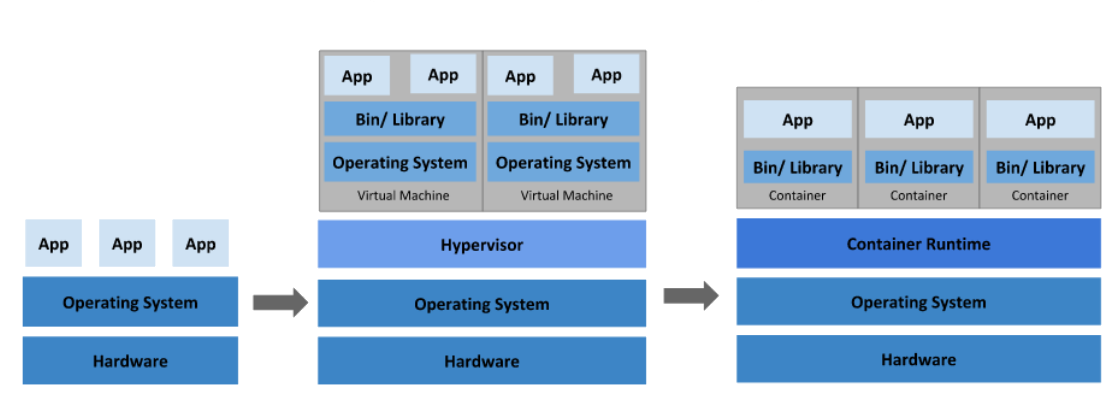
\includegraphics[width=1\textwidth]{vmsContainer.png}
      \end{center}
    \end{column}
  \end{columns}
\end{frame}

% -- 
% Revisão de Literatura - Cluster orquestrador de container
% -- 
\subsection{Cluster orquestrador de container}

\begin{frame}{Revisão de literatura- Cluster orquestrador de container}
  \begin{columns}
    \begin{column}{0.5\textwidth}
      \begin{itemize}
        \item Kubernetes\textregistered:
              \begin{itemize}
                \item Origem de 15 anos de trabalho da Google (Borg) %\cite{verma_large-scale_2015}
                \item Estrutura de objetos componentizados %\cite{kubernetes2022}
                      \begin{itemize}
                        \item Kube-apiserver
                        \item Kube-scheduler
                        \item Kube-controller-manager
                        \item Kubelet
                        \item Kube-proxy
                        \item Pod
                      \end{itemize}
              \end{itemize}
      \end{itemize}
    \end{column}
    \begin{column}{0.5\textwidth}  %%<--- here
      \begin{center}
        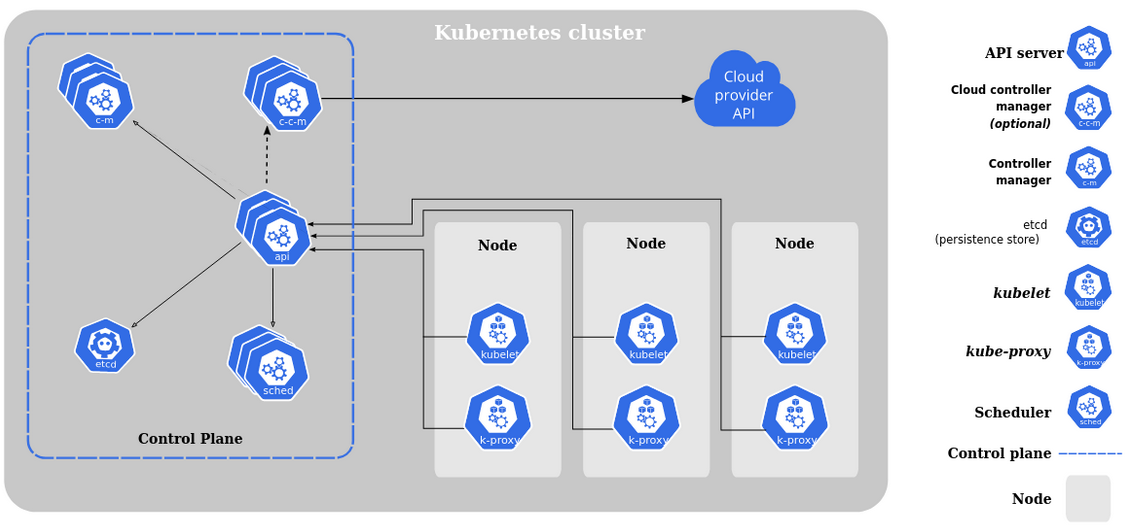
\includegraphics[width=1\textwidth]{kubeadm-node.png}
      \end{center}
    \end{column}
  \end{columns}
\end{frame}

% -- 
% Métodos
% -- 
\section{Método}

% -- 
% Método - Especificação dos nós integrantes cluster de baixo custo
% -- 
\subsection{Especificação dos nós integrantes cluster de baixo custo}

\begin{frame}{Método - Especificação dos nós integrantes cluster de baixo custo}
  \begin{columns}
    \begin{column}{0.5\textwidth}
      \begin{itemize}
        \item Cluster Simulado:
              \begin{itemize}
                \item Virtualização:
                      \begin{itemize}
                        \item Maquinas Virtuais (VMs) (\emph{Hypervisor} tipo 2)
                        \item Contêineres Aninhados (Docker In Docker, ou DinD)
                      \end{itemize}
                \item Especificações de hardware 1vCPU, 2 GB de RAM;
              \end{itemize}
        \item provisionamento em 2 etapas
        \item máquinas subutilizadas
        \item CAPEX
              
      \end{itemize}
    \end{column}
    \begin{column}{0.5\textwidth}  %%<--- here
      \begin{center}
        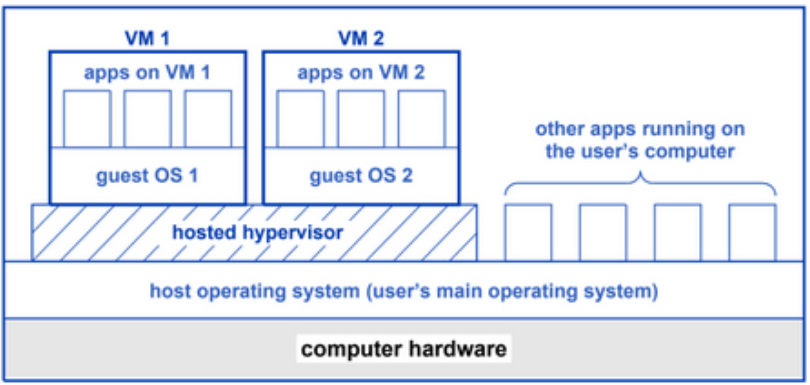
\includegraphics[width=1\textwidth]{vms.png}
      \end{center}
    \end{column}
  \end{columns}
\end{frame}


% -- 
% Método - Plataforma de orquestração de carga de trabalho
% -- 
\subsection{Plataforma de orquestração de carga de trabalho}

\begin{frame}{Método - Plataforma de orquestração de carga de trabalho}
  \begin{columns}
    \begin{column}{0.5\textwidth}
      \begin{itemize}
        \item Arquitetura sugerida para produção:
              \begin{itemize}
                \item Multi-master com Etcd junto ao nó master
              \end{itemize}
        \item Alta disponibilidade do cluster
        \item Recursos de hardware limitados
      \end{itemize}
    \end{column}
    \begin{column}{0.5\textwidth}  %%<--- here
      \begin{center}
        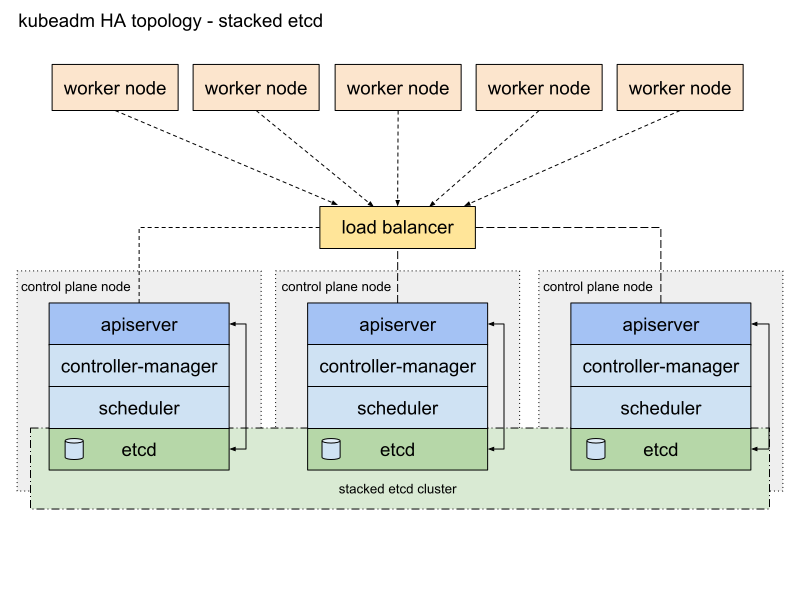
\includegraphics[width=1\textwidth]{kubeadm-ha-topology-stacked-etcd.png}
      \end{center}
    \end{column}
  \end{columns}
\end{frame}

\begin{frame}{Método - Plataforma de orquestração de carga de trabalho}
  \begin{itemize}
    \item Implantação da carga de Trabalho
          \begin{itemize}
            \item Container
            \item Parametrizável
            \item Volume compartilhado
          \end{itemize}
  \end{itemize}
\end{frame}

% -- 
% Método - Configuração e provisionamento do cluster
% -- 
\subsection{Configuração e provisionamento do cluster}

\begin{frame}{Método - Configuração e provisionamento do cluster}
  \begin{columns}
    \begin{column}{0.5\textwidth}
      \begin{itemize}
        \item[] O uso de gereniadores de configuração garantem o versionamento das configurações permitindo maio controle sobre as propriedades dos \emph{assets} gerenciados (Ansible\textregistered)
        \item \emph{Agentless}
        \item Idempotência
        \item Gerenciamento de inventário
        \item SSH - Escolha do algoritimo de criptografia %\cite{noauthor_rfc4254_nodate}
      \end{itemize}
    \end{column}
    \begin{column}{0.5\textwidth}
      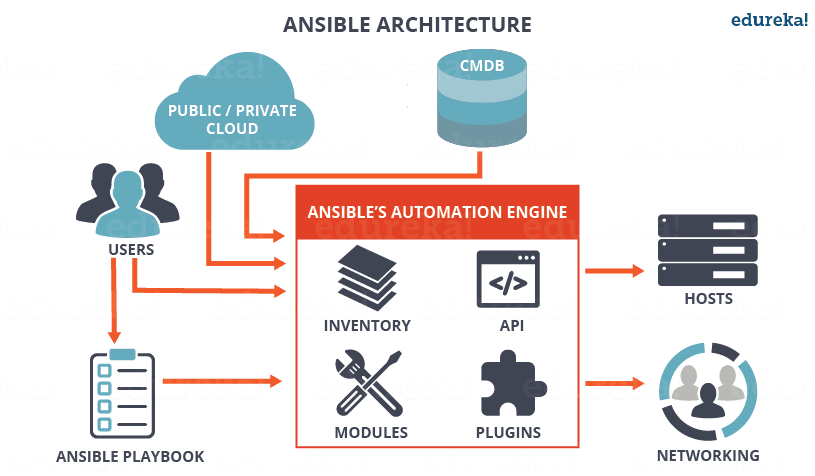
\includegraphics[width=1\textwidth]{ansible arch.png}
    \end{column}
  \end{columns}
\end{frame}

% -- 
% Método - Monitoramento
% -- 
\subsection{Monitoramento}

\begin{frame}{Método - Monitoramento}
  \begin{itemize}
    \item \emph{OpenTelemetry}
    \item \emph{Prometheus} Monitoramento de sistemas e Banco de dados de series temporais
    \item \emph{Grafana} - Dashboard e observabilidade
    \item Parametros de tempo, taxa de utilização de memoria e processamento
  \end{itemize}
\end{frame}


% -- 
% Método - Comparação entre tipos de virtualização
% -- 
\subsection{Comparação entre tipos de virtualização}

\begin{frame}{Método - Comparação entre tipos de virtualização}
  \begin{columns}
    \begin{column}{0.5\textwidth}
      
      \begin{itemize}
        \item Máquinas \emph{Host} e \emph{Guests} arquitetura x86
        \item Definição máquina \emph{host}:
              \begin{itemize}
                \item o \emph{host} será um laptop, contendo configuração de 4vCPUs e 16GB de RAM
                \item Hospedará as maquinas virtualizadas, pertencentes ao cluster
                      
              \end{itemize}
        \item Definição máquina \emph{guest}:
              \begin{itemize}
                \item como ja descrtio em 2 cenários: Virtualização completa, e em containers
                \item Nós do Cluster kubernetes (objeto de monitoramento)
              \end{itemize}
      \end{itemize}
    \end{column}
    \begin{column}{0.5\textwidth}
      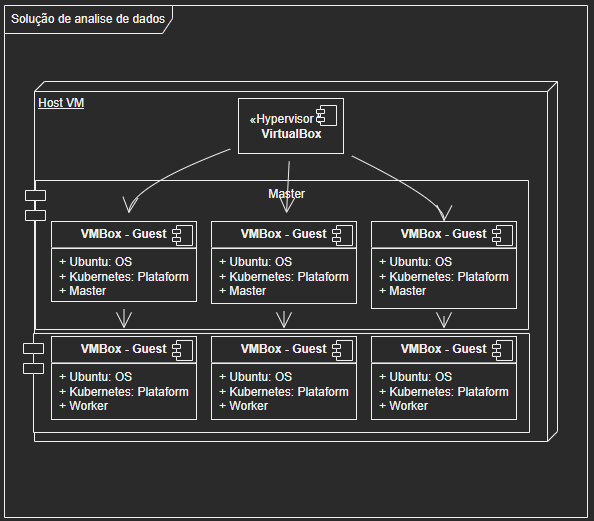
\includegraphics[[width=0.5\textwidth]{SCKET.png}
    \end{column}
  \end{columns}
  
  \framebreak
  \begin{itemize}
      
  \item macrobenchmark (system level benchmark) - Teste utizando uma solução avaliando tempo de execussão
  \item[] métricas de Desempenho (nós do cluster, \emph{guests}):
  \item Taxa de Utilização de CPU e Memória 
  \item Taxa de saturação de CPU e Memória
  \item[] Métricas de APM:
  \item Tempo Médio de todas as cargas de trabalho e variabilidade
  \item[] Método base utilizado para coleta de informações:
  \item Metodo USE de avaliação (Checklist Linux)
  \end{itemize}
  
\end{frame}


% -- 
% Método - Análise de dados
% -- 
\subsection{Análise de dados}

\begin{frame}{Método - Exemplo da Análise de dados}
  \begin{itemize}
    \item Vendas de Medicamentos Controlados e Antimicrobianos - Medicamentos Industrializados
    \item $530 \cdot 10^{6}$ linhas com mais de 70 GB
    \item Análise de tendência do consumo de azitromicina
    \item Caso base - comparação com processo de análise em \emph{bare metal} 8vCPU, 16 GB de RAM - totalizando o poder computacional total do cluster proposto
  \end{itemize}
\end{frame}

% -- 
% Método - Cronograma
% -- 
\subsection{Cronograma}

\begin{frame}[plain]
  \hspace*{-10mm}
  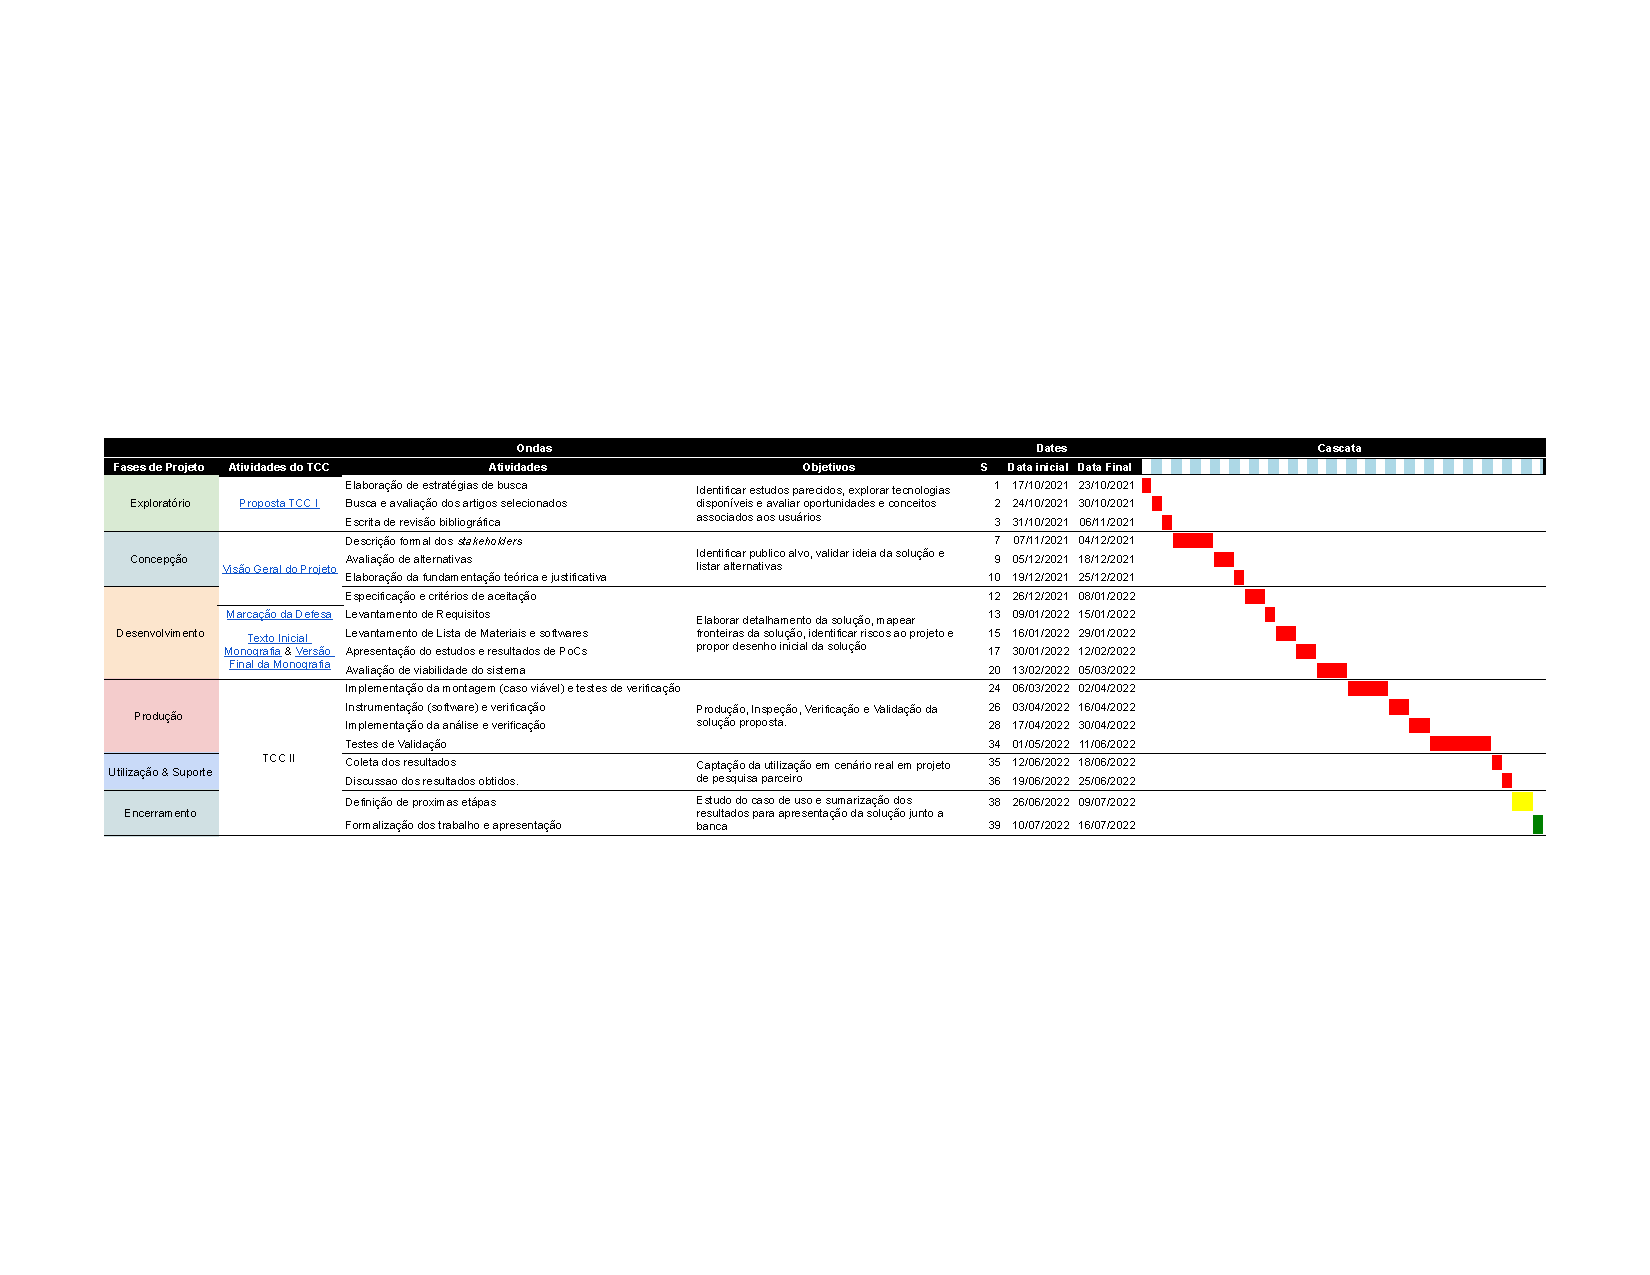
\includegraphics[width=\paperwidth]{TCC cronograma - Sheet1.pdf}
\end{frame}

% -- 
% Conclusão
% -- 
\section{Conclusão}

\begin{frame}{Conclusão}
  \begin{itemize}
    \item Avaliação de diferentes tipos de virtualização
    \item Seleção de plataforma de orquestração de cargas de trabalhos com base em requisitos e restrições
    \item Analise dos impactos socio-econômicos oriundos da restrição orçamentária a pesquisa de uma forma geral
    \item Desenho de uma estratégia de extração de informações relevantes de uma base de dados com volume considerável
    \item Entendimento da complexidade dos fatores considerados no processo de descisão em saúde
  \end{itemize}
  Trabalhos futuros contemplarão a implementação, testes e coletas de dados para avaliação comparativa das virtualizações propostas no ambiente simulado. Baseado nesses resultados pode se evoluir essa discussão na forma de recrutamento de computadores para o cluster de maneira a garantir o isolamento da maquina base.
\end{frame}


% -- 
% Disponibilidade dos recursos deste trabalho
% -- 
\section{Disponibilidade dos recursos deste trabalho}

\begin{frame}{Disponibilidade dos recursos deste trabalho}
  \begin{itemize}
    \item \href{https://github.com/felipefrocha/esufmg-tcc}{Github - Monorepo}
    \item \href{https://github.com/felipefrocha/esufmg-tcc/actions}{Pipeline}
  \end{itemize}
  Todos os componentes definidos neste trabalho estarão contidos em um ou mais repositórios públicos, sob a licença pública geral GNU versão 3, para livre acesso.
  
\end{frame}

% -- 
% Referências
% -- 
\begin{frame}[allowframebreaks]{Referências}
  \small
  %	\nocite{*}
  %    \bibliographystyle{apalike}
  \bibliography{Apresentacao}
\end{frame}


\begin{frame}
  \centering
  {\color{ros} OBRIGADO\\
    :)}
\end{frame}
\end{document}